\documentclass[12pt]{exam}
\usepackage{amsmath, amssymb, amsfonts, amsthm}
\usepackage{graphicx}
\usepackage{hyperref}
\usepackage{tikz}
\usepackage{tikz-qtree}
\usepackage[margin=2.5cm]{geometry}
% \usepackage{fancyhdr} 


\usepackage{arabtex}

\usepackage{polyglossia}

\setmainlanguage{english}
\setotherlanguage{urdu}
\newfontfamily\urdufont[Scale=1.25]{jameel.ttf}




% \geometry{margin=0.5in, footskip=0.5in}

% \printanswers

\newtheorem{corrolary}{Corrolary}
\newcommand{\classX}[1]{\ensuremath{\text{\textsf{\textbf{#1}}}}} 
\newcommand{\classP}{\classX{P}}
\newcommand{\classNP}{\classX{NP}}
\newcommand{\NPC}{\classX{NP-complete}}
\newcommand{\coNP}{\classX{coNP}}
\newcommand{\EXP}{\classX{EXP}}
\newcommand{\coEXP}{\classX{coEXP}}
\newcommand{\PSPACE}{\classX{PSPACE}}
\newcommand{\NPH}{\classX{NP-hard}}
\newcommand{\T}{\text{\textbf{T}}}
\newcommand{\F}{\text{\textbf{F}}}
% \newcommand{\gcd}{\text{gcd}}}


\newtheorem{theorem}{Theorem}
\newtheorem{lemma}{Lemma}
\newtheorem{proposition}{Proposition}
\newtheorem{corollary}{Corollary}
\newtheorem{definition}{Definition}






\begin{document}


\pagestyle{plain}

\begin{minipage}[l]{0.1\textwidth}
		\noindent
		
\includegraphics[width=1.8\textwidth]{math club logo.png}
	\end{minipage}
\hfill
\begin{minipage}[c]{0.7\textwidth}
    \begin{flushleft}
    \Huge\texturdu{ مدرسہ ریاضیات }
    \vspace*{0.5cm}
    \\\Large Lecture 05 -- The Travelling Salesperson
    \\\large Habib Math Club
    \end{flushleft}

\end{minipage}
\newline
\bigskip
%%%%%%%%%%%% Please compile with XeLaTeX %%%%%%%%%%%%
%%%%%%%%%%%% Enter your text here %%%%%%%%%%%%

\section{Become the Travelling Salesperson!}
You just moved into Turing Town and take up a job as a delivery driver for Lovelace and Co. You must drop off packages at 6 different houses every day and return home. Since you are a student and must save money, you track your fuel consumption. The first week, you try out different random routes and notice the different fuel costs. After a few weeks, you try to figure out what's the shortest possible route that visits each house exactly once and returns to your starting point? 

This challenge is called the \textbf{Travelling Salesperson Problem (TSP)}, a well-known and unsolved problem in computer science and mathematics.

\begin{center}
    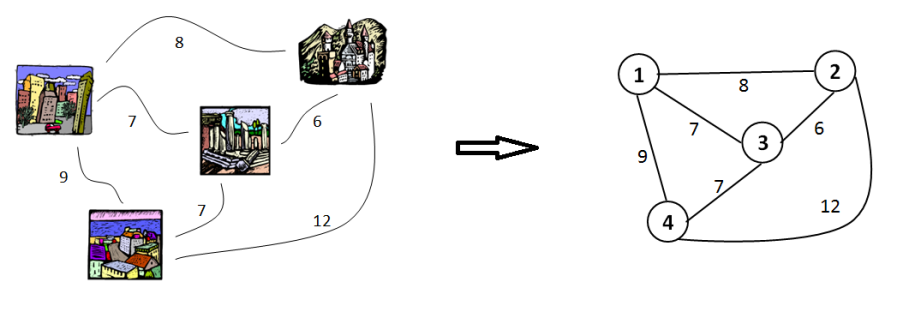
\includegraphics[width=1.0\textwidth]{Traveling salesman problem (TSP) 1.png}
\end{center}

\section{Graph Representation}
TSP is represented using a \textbf{weighted graph}, where:
\begin{itemize}
    \item \textbf{Vertices (Nodes)} represent the cities/houses.
    \item \textbf{Edges} represent roads connecting the cities.
    \item \textbf{Weights} on edges denote distances or costs.\\
\end{itemize}

\begin{center}
    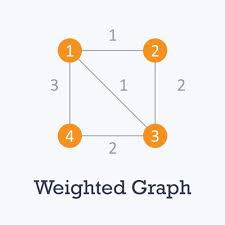
\includegraphics[width=0.3\textwidth]{weighted graph.jpeg}
\end{center}

\textbf{Hamiltonian Path:} A path that visits every vertex exactly once.\\

\textbf{Hamiltonian Cycle:} A Hamiltonian Path that returns to the starting vertex or the shortest cycle that visits every node (house) exactly once and returns to the start.

\section{Complexity of TSP}

Consider a small delivery map with 4 locations: A, B, C, D. The weights represent the fuel cost from one city to another.

\begin{center}
    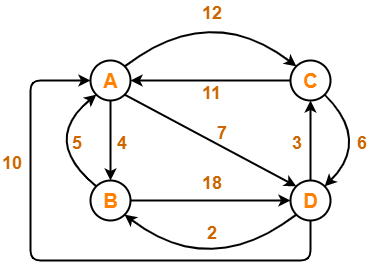
\includegraphics[width=0.5\textwidth]{travelling.png}
\end{center}

\begin{itemize}
    \item A valid TSP route starts and ends at the same point.
    \item It must visit every other location exactly once.
    \item For 4 points, the total number of unique tours is:
    \[
    (4-1)! = 3! = 6
    \]
\end{itemize}

Even for this small example, trying all possible tours is feasible, but the number of paths grows \textbf{factorially} with the number of cities.

\section{Brute Forcing Our Way?}

Suppose we have a fast computer that can check 1,000,000 routes per second.  
We can estimate computation time for $N$ locations using:
\[
(N-1)! \text{ routes to check.}
\]

\begin{center}
\begin{tabular}{c|c}
$N$ & Time to compute all routes \\
\hline
6 & Instantaneous \\
10 & 0.3 seconds \\
11 & 4 seconds \\
12 & 40 seconds \\
13 & 8 minutes \\
14 & 2 hours \\
15 & 1 day \\
25 & $\sim$2 million years \\
\end{tabular}
\end{center}

Brute force becomes impractical very quickly due to exponential (factorial) growth, and even computers take a long time to solve this problem. So much so we have an entire field in computer science relating to it!

\section{Common TSP Strategies and Algorithms}
Apart from the brute-force solution, other strategies include:
\begin{itemize}
    \item \textbf{Nearest Neighbor:} Choose the closest unvisited city at every step. It is fast, but doesn't always yield the best path.
    \item \textbf{Greedy Algorithm:} Pick the shortest available edge that doesn’t lead to a cycle or revisit a city.
    
There are other faster algorithms such as Dynamic and Linear Programming, which can reduce the time complexity of our algorithm. 

\end{itemize}

\section{Easy and Hard Problems in Computer Science}

As the name suggests, there are two kinds of problems in Computer Science:

\textbf{Easy Problems:}
\begin{itemize}
    \item Can be solved quickly (polynomial time, i.e the time required for a computer to solve a problem, where this time is a simple polynomial function of the size of the input).
    \item Examples: Sorting a list, finding the maximum number, simple search.
\end{itemize}

\textbf{Hard Problems:}
\begin{itemize}
    \item Require enormous time to solve as input grows.
    \item Examples: Travelling Salesperson Problem (TSP), code breaking, optimal packing, Sudoku.
\end{itemize}

Some easy problems like matrix multiplication or prime number checking can still require advanced methods.  
Some hard problems can sometimes be approximated or partially solved efficiently, but exact solutions are ineffective for large inputs.



\section{P vs NP and Complexity Theory}
What even is P and NP?

\begin{itemize}
    \item \textbf{P:} Problems that can be solved in \textbf{P}olynomial time.
    \item \textbf{NP:} Problems whose solutions can be verified in polynomial time, also called \textbf{N}on deterministic \textbf{P}olynomial time, even if finding that solution might be very hard. For example, Sudoku; solving a large puzzle might be hard, but once someone gives you a solution, it's easy to check that its correct. That's an NP problem.
\end{itemize}

The actual question is: Can P ever be equal to NP? 

\[
\boxed{
    \classP \overset{?}{=} \classNP
}
\]

If $P = NP$, it means all hard problems like TSP, Sudoku, protein folding, etc., can be solved efficiently. \textbf{Till now, no one knows the answer to this!} It’s one of the biggest open questions in mathematics.

\section{What Makes TSP Hard?}

TSP belongs to a class of problems called \textbf{NP-hard}, which means:
\begin{itemize}
    \item No known algorithm can solve all instances quickly, or in polynomial time.
    \item Even verifying the best possible answer is hard.
    \item Small increases in input size lead to exponential growth in computation.
\end{itemize}

TSP is also NP complete (both NP and NP Hard). \textbf{NP Complete} problems, like TSP and Sudoku, are the hardest problems in NP. If any one of them can be solved quickly, all NP problems can. \textbf{NP Hard} problems are at least as hard as NP problems, but might not even be checkable efficiently.\\
If someone gives you a route, it’s easy to compute its total distance and check if it’s under a given limit. But is TSP also P? Is there a fast (polynomial time) method to always find the shortest route?\\

In other words, if we generilse it, can we say: If it is easy to verify a solution (NP), is it also easy to find it (P)? If the answer is yes, i.e. P = NP, many hard problems, from scheduling deliveries to curing cancer, could suddenly become solvable.

To summarise:
\begin{center}
$P \subseteq NP \subseteq NP-Hard \subseteq Unsolvable$ 
\end{center}

\section{Real-World Applications}

TSP-like problems appear in:
\begin{itemize}
    \item Logistics and Delivery (e.g., Amazon, UPS)
    \item Ride-sharing routes (e.g., Uber, Careem)
    \item Circuit design (wiring shortest connections)
    \item Robotics path planning
    \item Astronomical scheduling (e.g., James Webb Space Telescope)
\end{itemize}



\begin{quote}
    \textit{"Simplicity is the final achievement. After one has played a vast quantity of notes and more notes, it is simplicity that emerges as the crowning reward of art." -Frédéric Chopin.}
\end{quote}







%%%%%%%%%%%% Replace with a Sher of your liking and uncomment this %%%%%%%%%%%%
% \vspace{2cm}
% \begin{center}
%     \texturdu{عشرتِ قطرہ ہے دریا میں فنا ہوجانا }
%     \\\texturdu{درد کا حد سے گزرنا ہے دوا ہو جانا }
%      \begin{flushleft}
%          \hspace*{4.5cm} (\texturdu{مرزا غالب })
%      \end{flushleft}
% \end{center}


\renewcommand\thefootnote{}


\renewcommand\thefootnote{\fnsymbol{footnote}}
\setcounter{footnote}{1}

% \nocite*{}

% \bibliographystyle{plain} 

% \bibliography{resource.bib}


\end{document}

% Template credit: Mujtaba Hassan





 


